\section{Überarbeitung der Dongle-App}
Der Prototyp der Dongle-App zeigte, dass die genannten Funktionalitäten technisch möglich sind. Für den Fußschalter sollen sie evaluiert und wenn nötig verbessert werden. Zudem sollen die verschiedenen Projekte, die sich durch die Implementierung des Fußschalters ergeben, getrennt werden.

\subsection{Trennung der Projekte}
Durch die Entwicklung des Fußschalter entstehen drei verschiedene Projekte, deren Code sich jeweils stark überschneidet. Dabei müssen Updates und Änderungen für eines der Projekte mit einem möglichst geringen Aufwand auch in die anderen übernommen werden. Insbesonders die Updates für das Framework der Hoffmann Group zur Abstraktion der \ac{BLE}-Schnittstelle nrf\_Base müssen, um die fehlerfreie Kommunikation des Fußschalters zu den \ac{HCT}-Werkzeugen sicherzustellen, in die Projekte des Dongles und des Fußschalters übernommen werden. Es wird in allen \ac{HCT}-fähigen Produkten eingesetzt und stetig weiterentwickelt und darf unter keinen Umständen den Code der anderen Projekte nicht beeinhalten. Auch muss berücksichtigt werden, dass die Projekte jeweils unterschiedliche Peripherie benötigen.\\
Folgende Peripherie darf dabei nur in den jeweiligen Projekten initialisiert werden:
\begin{itemize}
	\item nrf\_Base: \ac{UART}
	\item Dongle: Ein-Farben LED, \ac{USB}
	\item \ac{HCT}-FootSwitch: Fußtaster, Akku Power Management, Drei-Farben LED, \ac{USB}
\end{itemize}

Um diese Anforderungen zu erfüllen kann einerseits für alle drei Projekte eine eigene Codebasis geschaffen werden, die sich jeweils stark überschneiden und gesondert gepflegt werden müssen oder die selbe Codebasis für alle Projekte benutzt werden. Die erste Möglichkeit hat den Vorteil, dass sich die Entwicklung einfacher gestaltet, da auf diese Abhängigkeiten keine Rücksicht genommen werden muss. Zudem kann der Code stärker auf den Anwendungsfall optimiert werden, jedoch macht der enorme Arbeitsaufwand die gesonderten Codebasen zu unterhalten und auf dem neuesten Stand zu halten, diese Möglichkeit unpraktikabel. Des weiteren wurde aus Software architektonischen Gründen die Anwendung bereits gekapselt, wodurch die programmatische Abtrennung der Teile keinen außerordentlichen Entwicklungsaufwand erfordert.\\
Stattdessen muss aus der Main-Routine nur zwei Funktionsaufrufe mit Compilerschaltern abgetrennt werden, um den Code des Fußschalter bzw. Dongles vom nrf\_Base Projekt zu trennen. Zum einen der Initialisierungsaufruf und ein App-process Aufruf, da der Main-Loop als Dispatcher für die gesamte Anwendung fungiert. Im Central müssen die Datencallbacks, sowie im Connection State Callback die Aufrufe an die Dongle-App abgetrennt werden. Die Funktionalität der \ac{UART} stellte sich als wenig gekapselt heraus und musste an zahlreiche Stellen kleinteilig aus dem Fußschalterprojekt abgetrennt werden.\\ 
Das ambitioniertes Ziel war dabei, dass nach der Einführung der Compilerschalter das Binärfile des nrf\_Base Projekts identisch zu der vorangegangenen Version ohne Fußschalter sein sollte. Aus noch nicht geklärten Umständen ist das jedoch nicht der Fall.


\subsection{Verbesserung Verbindungsaufbau}
Im Ausgangszustand der Dongle-App werden lediglich zwei Zustände im Verbindungsaufbau abgebildet: ``unconnected'' und ``connected''. Aus der Zuordnung des Connection Handles, also dem Wechsel dieser Variable aus dem Default Wert 0xFFFF auf einen beliebigen anderen Wert, kann zusätzlich darauf geschlossen werden, dass die Service Discovery abgeschlossen wurde und mit der Subscription begonnen werden kann. Diese Abbildung des Verbindungsaufbaus ist mehrer Hinsicht unvollständig.\\
Der Zustand ``connected'' in der Dongle-App bildet den Zustand fehlerhaft ab. Er wird eingenommen, sobald ein erster Verbindungsaufbau durch die Anwendung angestoßen wurde. Zum diesen Zeitpunkt ist noch keine Kommunikation über die Scan Response hinaus erfolgt und folglich kann noch kein Connection Handle dem zu verbindenden Gerät zugeordnet werden. Im nrf\_Base Framework wird dieser Zustand, getriggert durch das korrespondieren Event, erst nach der initialen Kommunikation eingenommen und das Connection Handle ist bereits zugeordnet. Das ist ein entscheidender Unterschied, da ab diesem Zeitpunkt ein Verbindungsabbruch auftreten und nur über das Connection Handle nachvollzogen werden kann. Das kann dazu führen, dass im Werkzeug der Verbindungsaufbau fehlgeschlagen ist, jedoch in der Dongle-App das Gerät im Zustand ``connected'' ohne Connection Handle festhängt. Nicht nur wird dieses Wekrzeug nicht mehr vollständig verbunden, sondern solange es in diesem Zustand bleibt, wird bei keinem anderem Gerät ein Verbindungsaufbau angestoßen.\\
Wenn die Service Discovery ausgeführt wurde, wird in der Dongle-App mit diesem Event das Connection Handle zugeordnet und die Subscription angestoßen. Mit dieser Zuordnung ist in der Dongle-App das Gerät vollständig verbunden und die derzeitig eingestellte Messeinheit des Werkzeugs wird abgefragt. Dabei wird jedoch nicht darauf gewartet, dass das zu einer erfolgreichen Subscription korrespondieren Acknowledgement erhalten und der Zustand ``Subscription'' eingenommen wurde. Auch hier können bei einer fehlgeschlagenen Subscription Fehler in der Anwendung auftreten.\\
Die Zustände des Verbindungsaufbaus sollen jetzt korrekt und vollständig in der Anwendung abgebildet werden. Dabei wurde die Callback Funktionen bisher direkt im Eventhandler des Central aufgerufen. Diese Erweiterung hätte es erfordert, eine respektiven Callback in allen zugehörigen Events aufzurufen, was entgegen der Kapselung der Projekte geht. Jedoch gibt es im Central bereits eine ähnliche Funktionalität, die den Zustand des Central Moduls über \ac{UART} ausgibt und bereits in den Events des Verbindungsaufbaus aufgerufen wird. Sie wird nun erweitert, sodass falls der Compilerschalter für die \ac{USB}-App gesetzt ist, der Zustand des Moduls nicht über \ac{UART}, sondern an einen Callback der \ac{USB}-App überreicht wird. In der \ac{USB}-App wird der Zustand gespeichert und die dazugehörigen Folgeaktionen durchgeführt. Im Central Modul ist weiterhin nur ein einziger Aufruf einer \ac{USB}-App Funktion vonnöten, um die Zustände des Verbindungsaufbaus in der \ac{USB}-App abzubilden.

\begin{figure}[H] 
	\centering
	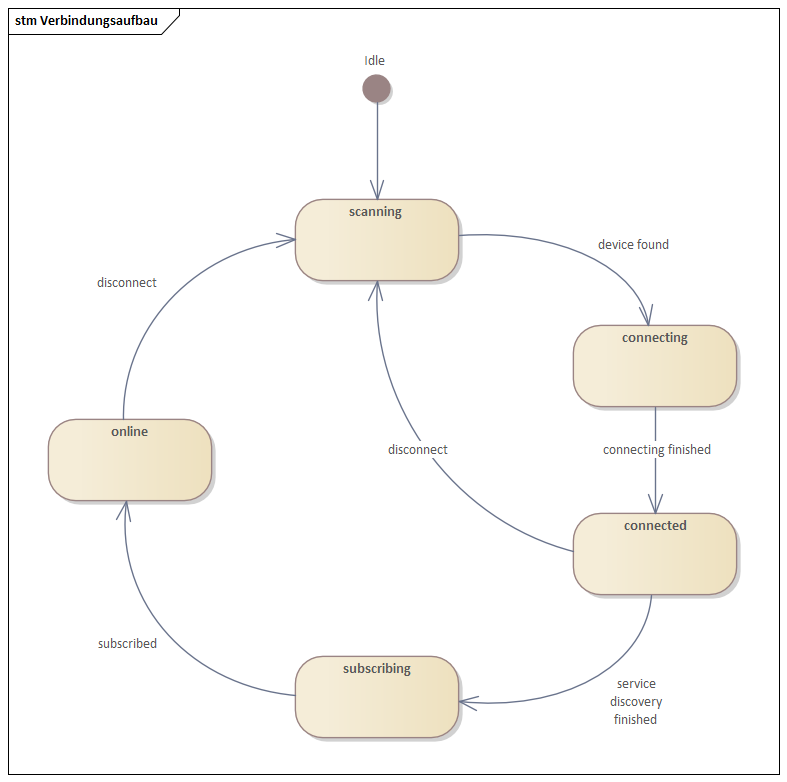
\includegraphics[width=\textwidth]{figures/Verbindungsaufbau.png}
	\caption{Zustandsdiagramm des Verbindungsaufbaus}
\end{figure}



\subsection{Optimierung Abfrage Messeinheit}
Jede Nachricht die über \ac{BLE} gesendet wird braucht Rechenleistung und Energie und steigt mit der Anzahl der verbundenen Geräte linear an. Im Ausgangszustand der \ac{USB}-Dongle App muss die Anwendung bei Werkzeug der Marke Holex jedes Mal, wenn sie ein Messergebnis erhält, die Einheit der Messung abfragen. Bei Drehmomentschlüsseln der Marke Garant wird ein Datenblock mit der Messeinheit kurz nach Erhalten des Messergebnisses empfangen. Diese Nachricht bezieht sich jedoch auf die derzeitig eingestellte Messeinheit, welche im Fall eines Arbeitsablaufs mit sich ändernden Einheiten, die Einheit für die nächste Messung ist. In diesem Fall gibt die \ac{USB}-Dongle App die falsche Einheit aus. Bei Geräten der Marke Holex wird nur bei einer Änderung der Messkonfiguration, diese übermittelt.\\
In beiden Fällen sendet das Werkzeug automatisch bei einer Änderung der Messkonfiguration einen Datenblock mit der Messeinheit an die Subscriber der \ac{HCT}-Charakteristik. Die Kontrolle der Messeinheit kann daher verbessert werden, indem die derzeitig eingestellte Messeinheit nach dem Verbindungsaufbau einmal abgefragt wird und für jedes verbundene Gerät gespeichert wird. Bei einer Änderung der Messeinheit erhält die Dongle-App die neue Messkonfiguration und aktualisiert die gespeicherte Einheit. Dadurch wird eine fehlerhafte Einheit in der Ausgabe vermieden, wird damit die Anzahl an Nachrichten der Dongle-App an das Messgerät verringert und die kritischen Ressourcen Rechenleistung und Energie geschont.

\begin{figure}[H] 
	\centering
	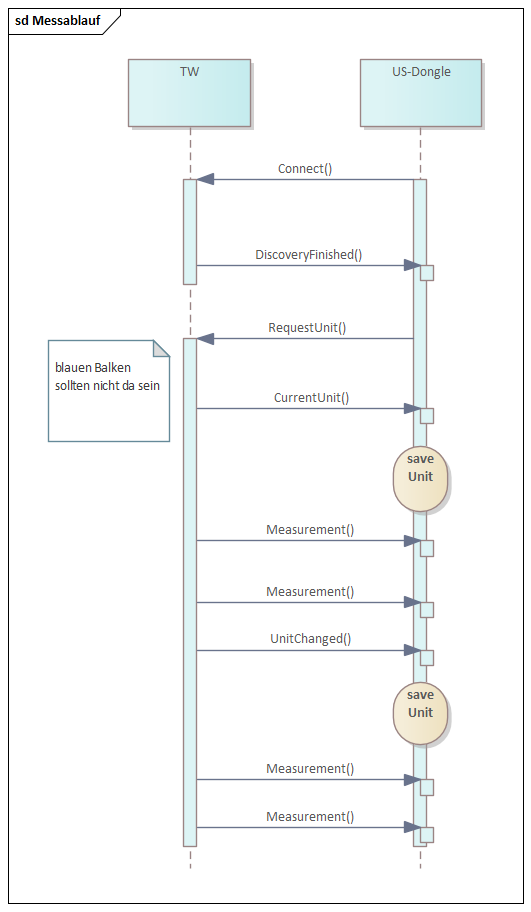
\includegraphics[width=\textwidth]{figures/Messablauf.png}
	\caption{Messablauf}
\end{figure}

